\documentclass[border=3pt,tikz]{standalone}
\usepackage{amsmath}
\usetikzlibrary{arrows.meta}
\usetikzlibrary{calc}
\begin{document}
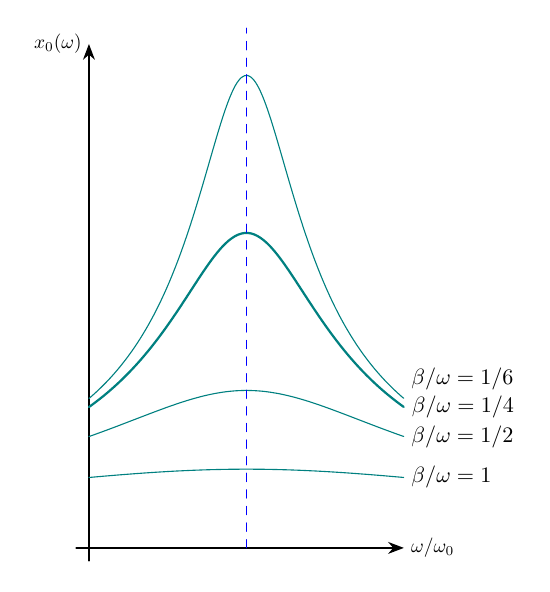
\begin{tikzpicture}[line cap=round, scale = 2]

    \draw [thick, -{Stealth[length=2mm]}, scale=0.8] (-0.1, 0) -- (2.5, 0) node [right, scale=0.7] {$\omega/\omega_0$};
    \draw [thick, -{Stealth[length=2mm]}, scale=0.8] (0, -0.1) -- (0, 4) node [left, scale=0.7] {$x_0(\omega)$};
    
    
    \draw[teal] plot[variable=\t,domain=0:2, samples=100, smooth,thick] ({\t}, {1.0/sqrt((1-\t)^2 + 4*1.0^2)}) node [right, scale=0.8, black] {$\beta/\omega = 1$};
    \draw[teal] plot[variable=\t,domain=0:2, samples=100, smooth,thick] ({\t}, {1.0/sqrt((1-\t)^2 + 4*0.5^2)}) node [right, scale=0.8, black] {$\beta/\omega = 1/2$};
    \draw[teal, thick] plot[variable=\t,domain=0:2, samples=100, smooth,thick] ({\t}, {1.0/sqrt((1-\t)^2 + 4*0.25^2)}) node [right, scale=0.8, black] {$\beta/\omega = 1/4$};
    \draw[teal] plot[variable=\t,domain=0:2, samples=100, smooth,thick] ({\t}, {1.0/sqrt((1-\t)^2 + 4*(1/6)^2)}) node [above right, scale=0.8, black] {$\beta/\omega = 1/6$};
    
    \draw[blue, dashed] (1,0) -- (1, 3.3);
    \end{tikzpicture}
\end{document}